\chapter{Introduction}\label{chap:intro}
\section{Background}
The boomerang attack is currently the most popular cryptanalysis method, it is based on the differential method, and was proposed by \cite{10.1007/3-540-48519-8_12}. It is a chosen plaintext attack and is used to analysis symmetric cryptography, compare to differential cryptanalysis, which provides a more efficient method to analyse more complex ciphers. Here is a brief introduction to the principle. Figure \ref{fig:boomerang} shows the design of basic boomerang analysis.  The boomerang attack attempts to generate a quartet structure at an intermediate value halfway through the cipher. 

\begin{figure}[hbt!]
    \centering
    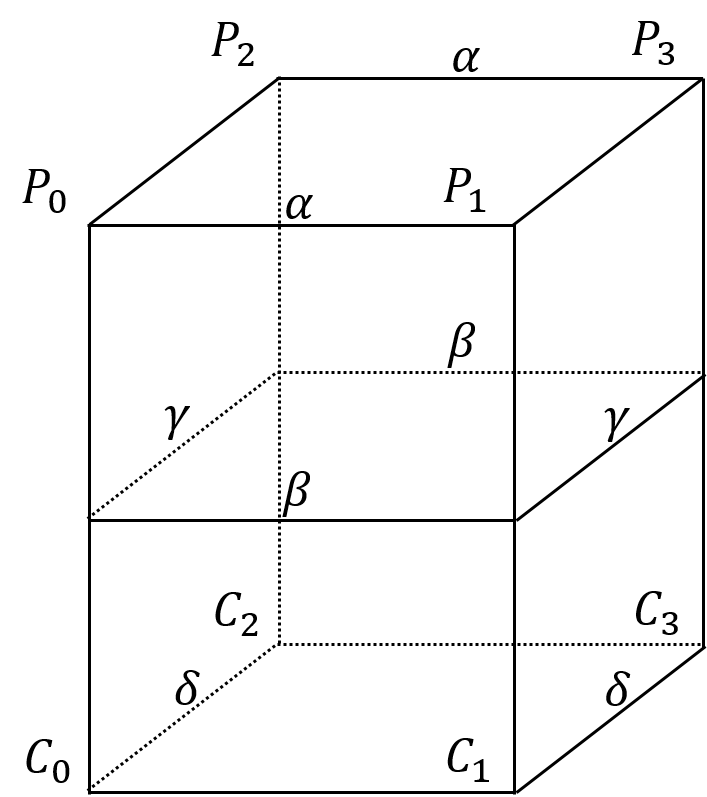
\includegraphics[width=45mm]{boomerang}
    \caption[Boomerang Attack Model]{Boomerang Attack Model}\label{fig:boomerang}
\end{figure}

The boomerang attack is widely used due to its power. However, \cite{5730575} raised concerns about the validity of the boomerang attack results that not all S-BOX ciphers boomerang distinguishers are reliable, for S-BOX based ciphers, two independently chosen differential trails can be incompatible, thus the probability of finding a right quartet can be zero and the same phenomenon was observed by \cite{10.1007/978-3-540-45146-4_12} as the middle round S-box trick. In order to solve this problem, \cite{10.1007/978-3-319-78375-8_22} proposed a new cryptanalysis tool called Boomerang Connectivity Table (BTC). Compared to the Difference Distributed Table (DDT), BTC can find better differential trails, the table [1] from the paper demonstrates the advantage. BTC has better efficiency than DDT, but it has only been used in practice on the S-BOX cipher so far, \cite{10.1007/978-3-319-78375-8_22} point out BTC may also be valid for modular addition ciphers.

With the development of IoT, more and more low-end devices are used, such as Smart Locks, there are large holdings of these devices, leading to an increasing need to provide security. Because these devices have the low computing power and run in a complex environment, several lightweight block ciphers were proposed. The KATAN family is based on modular addition, not S-BOX and was proposed by \cite{10.1007/978-3-642-04138-9_20}. Although it is subjected to many different types of analysis, it still provides security. The KATAN family contains six ciphers divide into two flavors, and all block ciphers share the 80-bits key size. KATAN is composed of three block ciphers, with 32,48, or 64-bits block size.  \cite{inproceedings} use an extended boomerang framework in related-key setting, to achieve the best results by far for KATAN48/64 in differential setting.




\section{Problem Statement}
As described in the previous section, the cryptanalysis based on boomerang has achieved good results \cite{inproceedings} on the KATAN cipher so far, but as \cite{5730575} point out, distinguishers based on boomerang analysis are not necessarily reliable. In other words, BTC \cite{10.1007/978-3-319-78375-8_22} can achieve a better result on S-BOX ciphers. So, there are some questions that need to be discovered:
\begin{enumerate}
    \item Whether BTC can apply non-S-BOX ciphers?
    \item How to improve the reliability of the result of the boomerang analysis of KATAN?
\end{enumerate}
Then, the following research questions will be answered in this work:
\begin{enumerate}
    \item What strategies can make BTC apply to ciphers based on modular operation, such as KATAN?
    \item How can achieve better results of boomerang analysis of KATAN than previous research using BTC?
\end{enumerate}


\section{Research Motivation}
With the rise of edge computing and the Internet of things, many devices need to save data locally, which also leads to high security for such devices. To improve the security of these devices without reducing performance, several lightweight cipers were proposed. KATAN is one example of them. It has withstood various cryptanalysis since it was proposed and still provides high security. This work uses it as a target cipher because it widely used in RFID devices, which represent a huge commercial value, and its analysis can further guarantee the security of the assets it protects. On the other hand, KATAN is a cipher based on modular addition, which can help this work to verify the adaptation of BTC on non-S-BOX ciphers. 

This work chose the boomerang attack as the cryptanalysis method because the efficiency of the boomerang attack was demonstrated in several research projects. This helped this work reduce the likelihood of failure, and due to the boomerang attack has become a research hotspot, many strategies which improve the efficiency of the attack were proposed. In conclusion, this work can achieve the better result by using the boomerang attack.

\section{Research Scope and Objectives}
\subsection{Research Scope}
This study consists of two parts. First, in cryptography, this work focus on block ciphers, which are symmetric-key cryptosystem.  Second, in cryptanalysis, this work focus on boomerang attack, which is an adaption of differential cryptanalysis. In short, the scope of this study is that boomerang attack on non-S-BOX block ciphers.

\subsection{Research Objectives}
According to this study research questions, the objectives of this research are summarized as follows:
\begin{enumerate}[noitemsep]
\item BTC be successfully applied on KATAN ciphers.
\item To improve the result of boomerang attack on KATAN ciphers by using BTC.
\end{enumerate}
Two objectives should be enough, and each objective should be measurable.

\section{Research Methodology}
This study has six steps, are shown in Figure \ref{fig:method}.
\begin{figure}[hbt!]
\centering
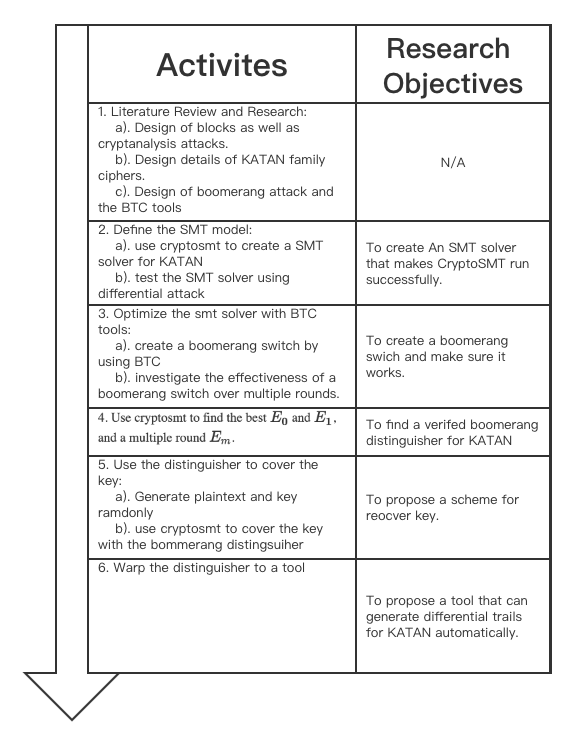
\includegraphics[width=150mm]{rm.png}
\caption[Research Framework]{Research Framework}\label{fig:method}
\end{figure}

\section{Research Contributions}


This study gets some contributions to cryptanalysis.

First, \cite{10.1007/978-3-319-78375-8_22} point out the BTC tools may be applied on ciphers based on modular addition operation, but it is not practiced. This study successfully demonstrates the BTC tools are not only used on ciphers based on S-BOX and useful to ciphers based on modular addition operations. The contribution can help cryptanalysts to improve their distinguisher of attack to ciphers based on modular operations.

This work also improves the probability of the boomerang distinguisher of KATAN. For KATAN48/64, this work was able to greatly improve upon the previous results to achieve the best result by for. The rules reflected in this distinguisher can help designers design ciphers better.

Last, this work proposed a tool that can generate distinguishers automatically, which can help improve the efficiency of attacking KATAN. Then summarize the contributions of this work as follows:

\begin{itemize}
\item A new strategy that can use BTC on ciphers based on modular addition operation.
\item Improve the probability of the distinguisher for KATAN.
\item A new cryptanalysis tool that can generate distinguishers for KATAN automatically.
\end{itemize}

\section{Thesis Outline}
Chapter 1 has provided an overview of the research including the introduction for KATAN and boomerang attack, and what is this study going to solve.

Next, Chapter 2 provides an in-depth review of prior work in the fields including block ciphers, KATAN, differential attack, boomerang attack and BTC.

Chapter 3 discusses the methodology involved in this research, we demonstrate the boomerang distinguisher search and key recovery attack on the KATAN family by using BTC. This is followed by Chapter 4 which analyses the findings and results, the BTC tools improve the probability of finding the right quartet.

Finally, this thesis concludes in Chapter 6 with a summary of finding and future works.
